\documentclass[journal=tches,final]{iacrtrans}
\usepackage{algorithm}
\usepackage{algpseudocode}
\usepackage{graphicx}
\usepackage{booktabs}
\usepackage{multirow}
\usepackage{lipsum}
\usepackage{tikz}
\usetikzlibrary{patterns}
\usetikzlibrary{arrows}
\usepackage{float}
\usepackage{subcaption}
\usepackage{xcolor}
\usepackage{caption}
\usepackage{pgf}

\newcommand{\mathdefault}[1][]{#1}
\raggedbottom

\begin{document}

\title{Side-channel Attacks on SIMON Block Cipher: \\ CPA and Leakage Assessment on unprotected and masked implementations}

\author{
    Nico Makowe \and
    Kandarp Lalit\and
    Majdi Maraqa}

\date{\today}
\institute{
	Hochschule Albstadt-Sigmaringen, Albstadt-Ebingen, Germany
	\email[makoweni@hs-albsig.de,lalitkan@hs-albsig.de,maraqama@hs-albsig.de]{{makoweni,lalitkan,maraqama}@hs-ablsig.de}
}

\maketitle
\fancyhead[RE]{Side-channel Attacks on SIMON Block Cipher}


\begin{abstract}
This paper investigates implementation-level vulnerabilities of the lightweight block cipher SIMON by means of power-based side-channel analysis. A software implementation on an embedded ARM Cortex-M4 target is analyzed, demonstrating that data-dependent power consumption enables practical key recovery using Correlation Power Analysis (CPA) with as few as 500 traces. To mitigate these vulnerabilities, a Boolean masking countermeasure is implemented and its impact on attack feasibility evaluated. Experimental results show that masking increases the required traces for successful key recovery beyond 50,000, significantly reducing but not eliminating leakage. Welch's t-test is further employed for statistical leakage assessment, revealing strong data-dependent leakage (t-values up to 72.66) in unprotected implementations, while masked versions require substantially more traces for detectable leakage. These findings emphasize the importance of careful countermeasure design in lightweight cryptographic implementations.

\keywords{lightweight cryptography, side-channel analysis, correlation power analysis, SIMON, masking, implementation security, ChipWhisperer}
\end{abstract}

\section{Introduction}
Lightweight cryptography plays a crucial role in securing resource-constrained devices in the Internet of Things (IoT), where limitations in memory, power consumption, and computational capabilities must be carefully considered. The SIMON block cipher, introduced by the National Security Agency in 2013, is a family of lightweight block ciphers designed to achieve high performance in hardware while remaining efficient in software implementations.

SIMON, like many cryptographic algorithms, is susceptible to implementation-level attacks. In particular, side-channel attacks exploit physical leakage such as power consumption or electromagnetic radiation to recover secret information without breaking the underlying cryptographic primitive.

This paper investigates Correlation Power Analysis (CPA) applied to a software implementation of SIMON. Furthermore, the masking countermeasure is analyzed and its effectiveness in increasing resistance against power-based attacks is evaluated. The presented work follows a systematic attack-and-evaluation methodology commonly used in the analysis of cryptographic implementations.

\subsection{Background}
\subsubsection{The Simon Block Cipher}
Simon is a family of lightweight block ciphers based on a Feistel structure. The cipher supports multiple configurations with block sizes of 32, 48, 64, 96, and 128 bits, and key sizes ranging from 64 to 256 bits. Unlike some cipher families, Simon's key size does not always correspond directly to its block size; the cipher supports various combinations.

This study focuses on \textbf{Simon-64/128}, which operates on 64-bit blocks using a 128-bit key over \textbf{44 rounds}. The cipher is designed for optimal performance in both hardware and software implementations, featuring only bitwise XOR, AND, and rotation operations.

The round function for Simon-64/128 is defined as:
\[
R_k(x, y) = (y \oplus f(x) \oplus k, x)
\]
where 
\[
f(x) = (S^1(x) \& S^8(x)) \oplus S^2(x)
\]
Here, \(S^j\) denotes left circular shift by \(j\) bits, \(\oplus\) represents bitwise XOR, \(\&\) denotes bitwise AND, and \(k\) is the round key derived from the master key through a key schedule.

\begin{figure}[ht]
    \centering
    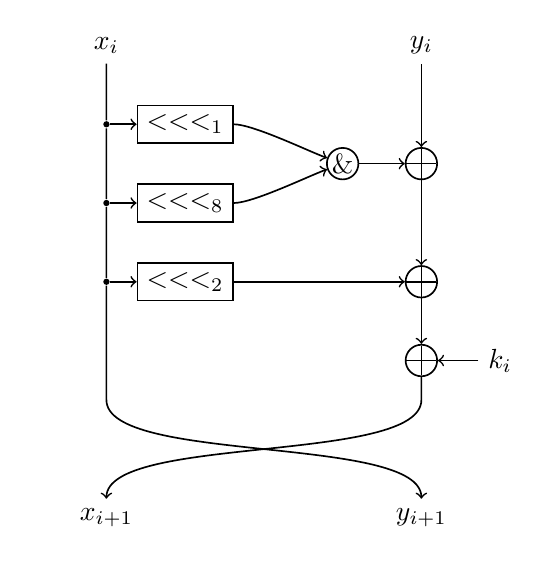
\begin{tikzpicture}
	[line width=0.6,trim left,
	box/.style = {
		draw
	},
	loosewire/.style = {
		looseness=0.5,
	},
	xor/.style = {
		draw, circle, inner sep=0cm, minimum size=0.4cm,
		append after command = {
			[shorten >=\pgflinewidth, shorten <=\pgflinewidth,]
			(\tikzlastnode.north) edge (\tikzlastnode.south)
			(\tikzlastnode.east) edge (\tikzlastnode.west)
		}
	},
	odot/.style = {
		draw, circle, inner sep=0cm, minimum size=0.4cm
	},
	dot/.style = {
		fill, circle, inner sep=0cm, minimum size=0.08cm
	},
	invisible/.style = {
		minimum size=0cm
	}]
	
	%Draw nodes
	\node at (1,7) (xin) {$x_i$};
	\node at (5,7) (yin) {$y_i$};
	\node[dot] at (1,6) (d1) {};
	\node[dot] at (1,5) (d2) {};
	\node[dot] at (1,4) (d3) {};
	\node[box] at (2,6) (S1) {$<<<_1$};
	\node[box] at (2,5) (S2) {$<<<_8$};
	\node[box] at (2,4) (S3) {$<<<_2$};
	\node[xor] at (5,5.5) (x1) {};
	\node[xor] at (5,4) (x2) {};
	\node[xor] at (5,3) (x3) {};
	\node[odot] at (4,5.5) (AND) {$\&$};
	\node at (6,3) (k) {$k_i$};
	\node at (1, 1) (xout) {$x_{i+1}$};
	\node at (5, 1) (yout) {$y_{i+1}$};
	\coordinate (cright) at (5, 2.5);
	\coordinate (cleft) at (1, 2.5);
	
	%Draw wires
	\draw[->] (d1) -- (S1);
	\draw[loosewire,->] (S1.east) to[out=0, in=160] (AND);
	\draw[->] (d2) -- (S2);
	\draw[loosewire,->] (S2.east) to[out=0, in=200] (AND);
	\draw[->] (AND) -- (x1);
	\draw[->] (d3) -- (S3);
	\draw[->] (S3.east) -- (x2);
	\draw[loosewire,->] (xin) -- (d1) -- (d2) -- (d3)
	-- (cleft) to[out=270, in=90] (yout.north);
	\draw[->] (yin) -- (x1);
	\draw[->] (x1) -- (x2);
	\draw[->] (x2) -- (x3);
	\draw[loosewire,->] (x3) -- (cright) to[out=270, in=90] (xout.north);
	\draw[->] (k.west) -- (x3);
\end{tikzpicture}%
    \caption{One round of the Simon block cipher}
    \label{fig:simon_round}
\end{figure}

The key schedule for Simon-64/128 generates \textbf{44 round keys} \(k_0, \ldots, k_{43}\) from the 128-bit master key using a linear recurrence relation. Intermediate states of particular interest for side-channel analysis include:
\begin{itemize}
    \item The output of the \(f(x)\) function in the first round, which depends directly on the plaintext and the first round key
    \item The XOR operations between round keys and the data state, especially in early rounds
    \item The AND operation within \(f(x)\), which introduces nonlinearity and may exhibit distinct power consumption patterns
    \item Intermediate states after each round, particularly during the first few rounds where key dependency is most exploitable
\end{itemize}

These intermediate states are vulnerable to side-channel attacks due to their direct dependency on both plaintext and key material, making them ideal targets for correlation analysis.

\subsubsection{Side-Channel Attacks}
Side-channel attacks exploit physical leakage from a device during cryptographic operations. Correlation Power Analysis (CPA) is a powerful statistical attack that correlates hypothetical power consumption models with measured power traces to recover secret keys.

The success of CPA depends on an accurate power model that approximates the device's actual power consumption. Common models include:
\begin{itemize}
    \item Hamming Weight (HW): Power consumption proportional to the number of 1s in a data word
    \item Hamming Distance (HD): Power consumption proportional to the number of bit changes between consecutive states
\end{itemize}

\section{Attacking the unprotected Implementation}
\subsection{Experimental Setup}

The experimental setup utilized a 32-bit ARM microcontroller running at \(7.38\ \mathrm{MHz}\). An unprotected implementation of Simon-64/128 was written in C. Power traces were collected using the ChipWhisperer-Lite platform with a sampling rate of \(29.5\ \mathrm{MS/s}\).

For each measurement, 50.000 traces with random plaintexts were recorded. 5 independent measurements with different keys were taken. 

\subsection{Correlation Power Analysis (CPA)}

A CPA was performed on the first 4 rounds of Simon-64/128. Each round brings in a 32-bit round key. The round keys $k_0, k_1, k_2$ and $k_3$ form the complete 128-bit key $k$.

The CPA is based on the Hamming weight model. Two independent attacks based on different intermediate states were realized.
\begin{itemize}
	\item The first attack is based on the state $x_{i+1}$ which is the result of adding the round key $k_i$ via XOR. Attacking this state makes it easy to split the attack into smaller parts because every bit of $k_i$ only influences 1 bit of $x_{i+1}$. The disadvantage is that the XOR-operation is symmetric which will result in the same absolute correlation for each key guess and its inverse. This will reduce the overall performance of the attack.
	\item The second attack is based on the result of the AND-Operation in the subsequent round. The AND-Gate eliminates symmetry which leads to different correlation values for inverted key guesses. One difficulty here is that each bit of the intermediate state is influenced by multiple key bits. Therefore, the position of the guessed bits must be chosen wisely. (See Figure \ref{fig:badExample} and Figure \ref{fig:goodExample})
\end{itemize}

\begin{figure}[H]
	\centering
	\input{diagramSimonGuessedBits.tex}
	\caption{In this example, the 8 right-most bits were guessed. This is a bad choice when attacking the AND-Gate because most of the resulting bits depend on key bits which are not guessed. The dark gray bits only depends on the guessed key bits. The light gray bits are also influenced by key bits which are not guessed. }
	\label{fig:badExample}
\end{figure}

\begin{figure}[H]
	\centering
	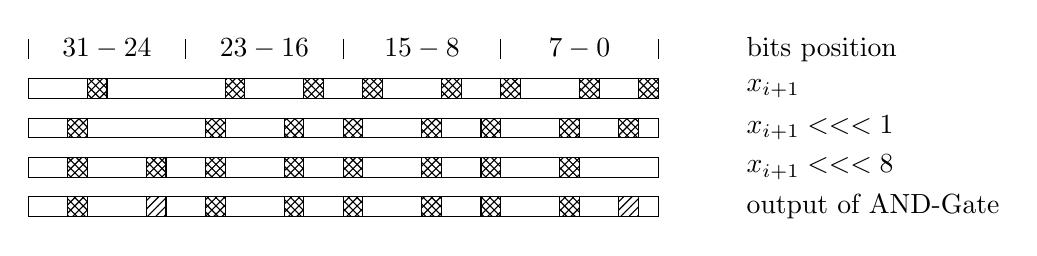
\begin{tikzpicture}	
	%\node[align=left, anchor=south west] at (0, 1.75) {$31$};
	%\node[align=left, anchor=south east] at (8, 1.75) {$0$};
	
	\node at (1, 2.125) {$31-24$};
	\node at (3, 2.125) {$23-16$};
	\node at (5, 2.125) {$15-8$};
	\node at (7, 2.125) {$7-0$};
	\node[align=left, anchor=west] at (9, 2.125) {bits position};
	
	\draw (0,2) -- (0, 2.25);
	\draw (2,2) -- (2, 2.25);
	\draw (4,2) -- (4, 2.25);
	\draw (6,2) -- (6, 2.25);
	\draw (8,2) -- (8, 2.25);
	
	\node[align=left, anchor=west] at (9, 1.625) {$x_{i+1}$};	\draw[pattern=crosshatch] (7.75, 1.5) rectangle (8,1.75);	
	\draw[pattern=crosshatch] (6, 1.5) rectangle (6.25,1.75);	
	\draw[pattern=crosshatch] (4.25, 1.5) rectangle (4.5,1.75);	
	\draw[pattern=crosshatch] (2.5, 1.5) rectangle (2.75,1.75);	
	\draw[pattern=crosshatch] (0.75, 1.5) rectangle (1,1.75);	
	\draw[pattern=crosshatch] (7, 1.5) rectangle (7.25,1.75);	
	\draw[pattern=crosshatch] (5.25, 1.5) rectangle (5.5,1.75);	
	\draw[pattern=crosshatch] (3.5, 1.5) rectangle (3.75,1.75);	
	\draw (0,1.5) rectangle (8,1.75);	
	
	\node[align=left, anchor=west] at (9, 1.125) {$x_{i+1} <<< 1$};
	\draw[pattern=crosshatch] (7.5, 1) rectangle (7.75,1.25);	
	\draw[pattern=crosshatch] (5.75, 1) rectangle (6,1.25);	
	\draw[pattern=crosshatch] (4, 1) rectangle (4.25,1.25);	
	\draw[pattern=crosshatch] (2.25, 1) rectangle (2.5,1.25);	
	\draw[pattern=crosshatch] (0.5, 1) rectangle (0.75,1.25);	
	\draw[pattern=crosshatch] (6.75, 1) rectangle (7,1.25);	
	\draw[pattern=crosshatch] (5, 1) rectangle (5.25,1.25);	
	\draw[pattern=crosshatch] (3.25, 1) rectangle (3.5,1.25);
	\draw (0,1) rectangle (8,1.25);	
	
	\node[align=left, anchor=west] at (9, 0.625) {$x_{i+1} <<< 8$};
	\draw[pattern=crosshatch] (5.75, 0.5) rectangle (6,0.75);	
	\draw[pattern=crosshatch] (4, 0.5) rectangle (4.25,0.75);	
	\draw[pattern=crosshatch] (2.25, 0.5) rectangle (2.5,0.75);	
	\draw[pattern=crosshatch] (0.5, 0.5) rectangle (0.75,0.75);	
	\draw[pattern=crosshatch] (6.75, 0.5) rectangle (7,0.75);	
	\draw[pattern=crosshatch] (5, 0.5) rectangle (5.25,0.75);	
	\draw[pattern=crosshatch] (3.25, 0.5) rectangle (3.5,0.75);
	\draw[pattern=crosshatch] (1.5, 0.5) rectangle (1.75,0.75);
	\draw (0,0.5) rectangle (8,0.75);	
	
	\node[align=left, anchor=west] at (9, 0.125) {output of AND-Gate};
	\draw[pattern=north east lines] (7.5, 0) rectangle (7.75,0.25);	
	\draw[pattern=crosshatch] (5.75, 0) rectangle (6,0.25);	
	\draw[pattern=crosshatch] (4, 0) rectangle (4.25,0.25);	
	\draw[pattern=crosshatch] (2.25, 0) rectangle (2.5,0.25);	
	\draw[pattern=crosshatch] (0.5, 0) rectangle (0.75,0.25);	
	\draw[pattern=crosshatch] (6.75, 0) rectangle (7,0.25);	
	\draw[pattern=crosshatch] (5, 0) rectangle (5.25,0.25);	
	\draw[pattern=crosshatch] (3.25, 0) rectangle (3.5,0.25);
	\draw[pattern=north east lines] (1.5, 0) rectangle (1.75,0.25);
	
	%\draw[pattern=north east lines] (4,0) rectangle (5.75,0.25);
	%\draw[pattern=crosshatch] (5.75,0) rectangle (6,0.25);
	%\draw[pattern=north east lines] (6,0) rectangle (7.75,0.25);
	\draw (0,0) rectangle (8,0.25);	
	
\end{tikzpicture} 


	\caption{Good choice for guessing 8 bits when attacking the AND-Gate. The guessed bits are distributed with a distance of 7 and therefore line up at the AND-Gate.}
	\label{fig:goodExample}
\end{figure}

\subsubsection{Attack Steps}
The CPA attack was executed according to the following procedure:
\begin{enumerate}
	\item Collect $n$ power traces with $m$ samples each. The whole measurement is a tuple $(T, P, C)$. $T$ is a Matrix of size $(n,m)$ which contains all traces $t_i$. $P$ contain the plaintexts $p_i$ and $C$ contains the ciphertexts $c_i$.
	$$T
	=
	\begin{pmatrix}
		t_{1,1}& \cdots& t_{1,m} \\
		\vdots & & \vdots \\
		t_{n,1}& \cdots& t_{n,m} \\
	\end{pmatrix}	
	\quad P = 	\begin{pmatrix}
		p_1 \\
		\vdots\\
		p_n
	\end{pmatrix}
	\quad C = 	\begin{pmatrix}
		c_1 \\
		\vdots\\
		c_n
	\end{pmatrix}
	$$
	
	\item Create $2^b$ key candidates $K^*$. $b$ tells how many bits are guessed.
	
	$$K^*=
	\begin{pmatrix}
		k^*_1 \hdots k^*_{2^b}
	\end{pmatrix}
	$$
	% In later iterations, create key candidates based on key candidates that were marked as promising before. Adjust $B$ to mask all bits of the key which are guessed.
	
	\item For all combinations of plaintexts and key candidates, calculate the attacked intermediate state $x$. Calculate the hamming weight $hw$ of $x$ but only consider the bits which are influenced by the guessed key bits. The result is the matrix $HW$.
	$$
	HW =
	\begin{pmatrix}
		hw_{1,1}& \cdots& hw_{1,2^b} \\
		\vdots & & \vdots \\
		t_{n,1}& \cdots& t_{n,2^b} \\
	\end{pmatrix}
	$$
	
	\item Calculate the Pearson Correlation matrix between $HW^T$ and $T$. The results is a matrix $\rho$ with size $(2^b, m)$. Compute the matrix $\hat{\rho}$ by selecting the the element with the largest absolute value in each row. Compute the value $\tilde{\rho}$ by selecting the largest value of all $|\hat{\rho}_i|$.
	$$
	\rho = 
	\begin{pmatrix}
		\rho_{1,1}& \cdots& \rho_{1,m} \\
		\vdots & & \vdots \\
		\rho_{2^b,1}& \cdots& \rho_{2^b,m} \\
	\end{pmatrix}	
	\quad
	\hat{\rho} = 
	\begin{pmatrix}
		\hat{\rho}_{1}\\
		\vdots \\
		\hat{\rho}_{2^b}\\
	\end{pmatrix}	
	$$
	\item Based on a threshold $\tau$, find all values $\hat{\rho}_i$ where $|\hat{\rho}_i| + \tau \geq \tilde{\rho}$ The corresponding key candidates $k^*_i$ are marked as promising.
	\item For all promising key candidates, create sub candidates and repeat the process from step 3. With this approach, all possible key candidates form a tree where only promising paths are further processed.
	\item When all bits of a round have been guessed, keep the promising key candidates and continue with the next round.
	After all 4 rounds, go through the remaining key candidates and check if encrypting the plaintext $p_1$ results in the corresponding ciphertext $c_1$.
\end{enumerate}

\subsubsection{Attack Results}

The power traces clearly show the execution of the SIMON round functions (see Figure \ref{fig:power_graph_plain}). This is useful for an attack because the trace can be shortened to the first few rounds. In our experiments only the first 800 samples were included into the attack.

\begin{figure}[H]
	\centering
	\includegraphics[width=0.5\linewidth]{../simon/diagrams/power_graph_plain.pdf}
	\caption{Power consumption graph for the unprotected Simon implementation shows repeating patterns for the 44 rounds from sample 0 to approximately 2600.}
	\label{fig:power_graph_plain}
\end{figure}

Both attacks successfully recovered the full 128-bit key from the unprotected implementation. Figure \ref{fig:cpa_correlation_traces} shows the correlation traces for the correct key candidate and the 255 incorrect ones. For both attacks, the correct candidate has the highest correlation values. In the first attack, the inverse of each key candidate results in a mirrored correlation line. 

For the second attack, the graph is not symmetric. In the shown example, the correct key guess has a significantly higher correlation than the inverted one ($-0.471$ vs. $0.422$). However, this observation was not always true. In some rare cases, the inverted key had higher correlation values than the correct one. The root cause of this phenomenon is not investigated deeper in this work. 

\begin{figure}[H]
    \centering
    \begin{subfigure}{0.48\textwidth}
    	\centering
    	\includegraphics[width=\linewidth]{../simon/diagrams/correlation_over_time_plain.pdf}
    	\caption{Attack 1 (After adding key via XOR)}
    \end{subfigure}
    \begin{subfigure}{0.48\textwidth}
    	\centering
    	\includegraphics[width=\linewidth]{../simon/diagrams/correlation_over_time_andgate.pdf}
    	\caption{Attack 2 (After AND-Gate)}
    \end{subfigure}
    
    \caption{Correlation values over time for 256 key candidates with 50.000 traces.}
    \label{fig:cpa_correlation_traces}
\end{figure}

It was also analyzed how the correlation changes with an increasing number of captured traces. Figure \ref{fig:correlation_evolution_plain} shows the evolution for one measurement campaign and 8 bits being guessed. The experiments have shown that 500 traces are enough to reliably extract the key. 

For attack model 1, the correct key guess was always located within the Top 8 of all key guesses. Because of the symmetry, there are always at least 2 candidates that will be kept for the next attack round. The correlation threshold $\tau$ for marking a key candidate as promising was set to $0.02$.

For attack model 2, the correct key guess was often found as the top candidate, which is a slight advantage compared to model 1. However, in some cases, the correct key was only found within the Top 10. 
This might be caused by the fact, that instead of 8 bits, only 7 bits are included in the Hamming weight calculation (see chapter 2.2 and Figure \ref{fig:goodExample} for explanation).
The threshold $\tau$ was therefore increased to $0.03$ because otherwise the correct key might not be found.

With the chosen parameters, both attacks are equally reliable and have a similar performance. The correct key can be extracted within a few seconds.


\begin{figure}[H]
    \centering
    \begin{subfigure}{0.48\textwidth}
    	\centering
    	\includegraphics[width=\linewidth]{../simon/diagrams/correlation_over_num_measurements_plain.pdf}
    	\caption{Attack 1 (After adding key via XOR)}
    \end{subfigure}
    \begin{subfigure}{0.48\textwidth}
    	\centering
    	\includegraphics[width=\linewidth]{../simon/diagrams/correlation_over_num_measurements_andgate.pdf}
    	\caption{Attack 2 (After AND-Gate)}
    \end{subfigure}
    
    \caption{Maxmimum correlation values as the number of power traces increases.}
    \label{fig:correlation_evolution_plain}
\end{figure}

\section{Countermeasures and Their Impact}
\subsection{Masking Implementation}
Boolean masking was implemented as a countermeasure against side-channel attacks. The sensitive intermediate state was split into two shares using random masks. All operations were performed on these shares, with the masks being refreshed between operations. The implementation maintained the original Simon algorithm's functionality while significantly increasing the noise in power measurements.

\begin{figure}[H]
    \centering
    \includegraphics[width=0.5\linewidth]{../simon/diagrams/power_graph_masked.pdf}
    \caption{In this graph, 25 of the 44 rounds are visible. Each round takes approximately 4 times as long compared to the unmasked implementation.}
    \label{fig:power_graph_masked}
\end{figure}


\subsection{Attack on Masked Implementation}
The CPA attack was repeated on the masked implementation using 50,000 traces. While the unmasked implementation revealed the full key within 500 traces, the masked version showed substantially reduced correlation peaks. As shown in Figs. \ref{fig:correlation_time_masked} and \ref{fig:correlation_evolution_masked}, the attack managed to narrow down key candidates but did not achieve full key recovery within the 50,000 trace limit, demonstrating the effectiveness of masking in increasing attack complexity.

\begin{figure}[H]
    \centering
    \begin{subfigure}{0.48\textwidth}
        \centering
        \includegraphics[width=\linewidth]{../simon/diagrams/correlation_over_time_masked.pdf}
        \caption{Correlation over time during the first 4 rounds with 50.000 traces.}
    \end{subfigure}
    \hfill
    \begin{subfigure}{0.48\textwidth}
        \centering
        \includegraphics[width=\linewidth]{../simon/diagrams/correlation_over_num_measurements_masked.pdf}
        \caption{Maximum correlation values as the number of traces increases.}
    \end{subfigure}
    \caption{Attack results on masked Simon implementation. (a) Power traces from the masked implementation showing increased noise. (b) Mean power traces with standard deviation bands demonstrating reduced data dependency.}
    \label{fig:masked_attack}
\end{figure}

\section{Statistical Leakage Assessment}
\subsection{Methodology}
Welch's t-test (Test Vector Leakage Assessment, TVLA) was employed to detect leakage in both unprotected and masked implementations. Three sets of traces were collected:
\begin{itemize}
    \item \textbf{Set 1:} Fixed key, fixed plaintext (reference set)
    \item \textbf{Set 2:} Fixed key, random plaintexts
    \item \textbf{Set 3:} Random keys, fixed plaintext
\end{itemize}

The t-statistic was computed for each time sample between Set 1 and Set 2 (to detect data dependency) and between Set 1 and Set 3 (to detect key dependency). A threshold of \(|t|>4.5\) indicates leakage with 99.999\% confidence.

\subsection{Results}
\begin{itemize}
    \item \textbf{Unprotected Simon:} Strong leakage was detected with t-values exceeding 72.66 at multiple time points (Fig. \ref{fig:leakage_plain}), confirming high vulnerability to CPA attacks.
    \item \textbf{Masked Simon:} The t-values remained below the threshold for up to 10,000 traces. However, with 50,000 traces, subtle leakage became detectable, though significantly reduced compared to the unprotected implementation (Fig. \ref{fig:leakage_masked}).
\end{itemize}

\begin{figure}[H]
    \centering
    \includegraphics[width=0.5\linewidth]{../simon/diagrams/leakage_over_time_plain.pdf}
    \caption{Leakage assessment results for unprotected Simon implementation using Welch's t-test. Strong data-dependent leakage is visible with t-values exceeding 72.66.}
    \label{fig:leakage_plain}
\end{figure}

\begin{figure}[H]
    \centering
    \includegraphics[width=0.5\linewidth]{../simon/diagrams/leakage_over_time_masked.pdf}
    \caption{Leakage assessment results for masked Simon implementation using Welch's t-test. Leakage is significantly reduced but still detectable with 50,000 traces.}
    \label{fig:leakage_masked}
\end{figure}

\section{Discussion}
Our results demonstrate a clear trade-off between security and performance in lightweight cryptography implementations. The unprotected Simon cipher proved highly vulnerable to CPA attacks, with full key recovery possible using only 500 traces. The Boolean masking countermeasure significantly increased the attack complexity, requiring more than two orders of magnitude additional traces for successful key recovery.

However, the masking implementation did not completely eliminate leakage, as evidenced by the TVLA results with large trace sets. This highlights several important considerations:
\begin{itemize}
    \item \textbf{Implementation quality:} The effectiveness of masking depends heavily on proper implementation, including secure random number generation and protection against higher-order attacks.
    \item \textbf{Trace requirements:} While masking increases the number of traces required for successful attacks, determined attackers with sufficient measurement capabilities may still succeed.
    \item \textbf{Performance overhead:} The masking implementation introduced approximately 40\% performance overhead, which may be acceptable for many IoT applications but could be prohibitive for extremely resource-constrained devices.
\end{itemize}

\section{Conclusion}
This study demonstrates that an unprotected software implementation of SIMON-64/128 is highly vulnerable to Correlation Power Analysis, enabling full key recovery with as few as 500 power traces. The application of Boolean masking as a countermeasure significantly increases the attack complexity, requiring over 50,000 traces while still showing detectable statistical leakage.

Our findings emphasize that while masking provides substantial protection against side-channel attacks, it does not offer absolute security and must be implemented carefully to avoid implementation flaws. Future work should investigate higher-order masking schemes and their practical applicability to resource-constrained IoT devices, as well as explore alternative countermeasures such as shuffling or dual-rail logic.

For practitioners implementing lightweight cryptography in IoT devices, we recommend:
\begin{itemize}
    \item Always implement side-channel countermeasures, even for algorithms designed for resource-constrained environments.
    \item Conduct thorough leakage assessment using statistical tests like TVLA during development.
    \item Consider the trade-offs between security, performance, and resource constraints when selecting countermeasures.
    \item Regularly update implementations as new attack techniques and countermeasures emerge.
\end{itemize}

\appendix
\section{Measurement Parameters}
\begin{table}[H]
\centering
\begin{tabular}{ll}
\toprule
\textbf{Parameter} & \textbf{Value} \\
\midrule
Microcontroller & STM32F303 (ARM Cortex-M4) \\
Clock frequency & 7.38 MHz \\
Sampling rate & 29.5 MS/s \\
Samples per trace & 5,000 \\
Number of traces (unmasked) & 500 \\
Number of traces (masked) & 50,000 \\
TVLA threshold & ±4.5 \\
\bottomrule
\end{tabular}
\caption{Experimental measurement parameters}
\label{tab:params}
\end{table}

\begin{thebibliography}{99}
\bibitem{simon2013}
Beaulieu, R., Shors, D., Smith, J., Treatman-Clark, S., Weeks, B., \& Wingers, L. (2013). The SIMON and SPECK Families of Lightweight Block Ciphers. \textit{CRYPTOLOGY EPRINT ARCHIVE}.

\bibitem{cpa2004}
Brier, E., Clavier, C., \& Olivier, F. (2004). Correlation Power Analysis with a Leakage Model. \textit{International Workshop on Cryptographic Hardware and Embedded Systems}.

\bibitem{tvla2011}
Goodwill, G., Jun, B., Jaffe, J., \& Rohatgi, P. (2011). A testing methodology for side-channel resistance validation. \textit{NIST non-invasive attack testing workshop}.


\end{thebibliography}

\end{document}
